\documentclass[12pt]{article}
\usepackage{polski}
\usepackage[utf8]{inputenc}
\usepackage{fullpage}
\usepackage{tabto}
\usepackage{graphicx} 
\usepackage{float}
\usepackage{caption}
\usepackage{indentfirst}




\linespread{1.3}
\begin{document}
%---------------------------------------------------------
%					Strona Tytułowa
%---------------------------------------------------------
\begin{titlepage}
%-----------------------Tytuł-----------------------------
\newcommand{\LINE}{\rule{\linewidth}{0.7mm}}
\center
\LINE \\[0.5cm]
\Huge\textsc{Cyfrowa historia pojazdu}\\ [5mm]
\normalsize\textsc{Zastosowanie Informatyki w Gospodarce}  \\[0.5cm]
\LINE \\[3cm]
%----------------------Nazwiska---------------------------
\begin{minipage}{0.5\textwidth}
\begin{flushleft} \large
\emph{Autorzy:}
		\\Grzegorz Milaszkiewicz %226110
		\\Mateusz Ożóg %226125
		\\Igor Kurek
		\\Piotr Wodzyński
		\\Maciej Kucia 
\end{flushleft}
\end{minipage}
~
\begin{minipage}{0.45\textwidth}
\begin{flushright} \large
\emph{Prowadzący:} \\
dr inż. Marek Woda
\end{flushright}
\end{minipage}\\[2cm]
%----------------------Stopka-----------------------------
\vfill
\center Wrocław 2019
\end{titlepage}

%---------------------------------------------------------
%					Spis treści
%---------------------------------------------------------
\renewcommand{\contentsname}{Spis treści}
\tableofcontents
\newpage

%---------------------------------------------------------
%					Część pierwsza
%---------------------------------------------------------
\section{Temat projektu}
Uzasadnienie biznesowe (skąd pomysł / dlaczego / czy jest innowacyjny i w jakim zakresie)\\

Tematem projektu jest system umożliwiający dokumentowanie historii pojazdów. Obecnie rynek samochodów używanych jest kojarzony z tak zwanym "kręceniem liczników", czyli zmniejszaniem faktycznego przebiegu pojazdu w celu podwyższenia jego wartości. Usługa korekty licznika jest stosunkowo tania i trudno wykrywalna. Najbardziej na tego typu zabiegach cierpią uczciwi posiadacze samochodów, którzy mają trudność w sprzedaży pojazdów z oryginalnym przebiegiem. System do dokumentowania historii pojazdów umożliwiłby uczciwym sprzedawcom na podniesienie wartości swoich pojazdów. Pomysł dokumentowania historii pojazdu nie jest pomysłem innowacyjnym. Na rynku jest wiele aplikacji umożliwiających zapisywanie historii pojazdów jednakże żadna z nich nie weryfikuje wprowadzanych danych. System\textit{ Cyfrowa historia pojazdu} będzie posiadał podobne funkcjonalności co inne aplikacje dostępne na rynku, lecz dodatkowo wymaga wprowadzenia przebiegu pojazdu przy każdym wpisie do bazy danych. Kolejną funkcjonalnością potwierdzającą dodanie wpisu będzie możliwość dodania zdjęcia (na przykład zdjęcia licznika pojazdu).




%---------------------------------------------------------
%					Część druga
%---------------------------------------------------------
\newpage
\section{Zakres projektu}
\subsection{Cele}
Celem projektu jest stworzenie systemu umożliwiającego dokumentowanie histroii pojazdów. Głównym zadaniem jest napisanie aplikacji mobilnej i webowej, która będzie przyjazna dla użytkownika. Aplikacja będzie przeznaczona dla właścicieli pojazdów oraz dla serwisów samochodowych. 
\subsection{Ryzyka}
Projektując taki system należy liczyć się z nieuniknionym ryzykiem. Głównym niebezpieczeństwem projektowanego systemu jest niskie lub całkowity brak zainteresowania ze strony użytkowników. Jest to dość realne zagrożenie z uwagi na mnogość tego typu aplikacji, które pomimo braku weryfikacji wprowadzanych informacji są o wiele bardziej wypromowane. 

Kolejnym ryzykiem jest opóźnienie w wykonywaniu pracy. Jest to istotne niebezpieczeństwo, które może wyniknąć ze zbyt dużej ilości funkcjonalności oraz z niedostatecznej wiedzy programistycznej w wybranych technologiach. 

Następnym ryzykiem jest zmiana założonych na początku funkcjonalności podstawowych systemu. Każda nieprzewidziana zmiana niesie za sobą spore konsekwencje. Nawet niewielka modyfikacja założeń projetkowych może spowodować opóźnienia w planowanym ukończeniu projektu.

\subsection{Funkcjonalności podstawowe i rozszerzone}

W tabeli 1-X zostały przedstawione podstawowe funkcjonalności systemu.

%----------------------REJESTRACJA------------------------------------
\begin{table}[H]
\begin{center}
\captionof{table}{Karta wymagań dla funkcjonalności \textit{Rejestracja konta}} 
	\begin{tabular}{|p{0.18\linewidth}|p{0.72\linewidth}|}%{|l|l|}
	\hline
	Id wymagania 	& 1 				\\ \hline
	Nazwa			& Rejestracja konta \\ \hline
	Opis & Aplikacja powinna zarejestrować użytkownika po wypełnieniu
formularza rejestracyjnego\\ \hline
	Przesłanka & Możliwość dodawania nowych użytkowników  \\ \hline
	Ograniczenia i~warunki & Rejestracja nowych użytkowników może odbyć się tylko po potwierdzeniu adresu e-mail  \\ \hline
	Dane wejściowe & Typ konta: 1. Właściciel pojazdu, 2. Serwis \\
	&  1. Imię, nazwisko, rok urodzenia, email, hasło \\
	& 2. Nazwa serwisu, adres (ulica, kod pocztowy, miasto), adres email, hasło  \\ \hline
	Wynik & Dodanie nowego użytkownika do systemu \\ \hline
	Źródło danych wejściowych & Użytkownik (Właściciel pojazdu, Serwis samochodowy, Osoba zewnętrzna) \\ \hline
	Przeznaczenie & Każdy nowy użytkownik \\ \hline
	\end{tabular}

\end{center}
\end{table}

%----------------------LOGOWANIE------------------------------------
\begin{table}[H]
\begin{center}
\captionof{table}{Karta wymagań dla funkcjonalności \textit{Logowanie}} 
\end{center}
	\begin{tabular}{|p{0.18\linewidth}|p{0.72\linewidth}|}%{|l|l|}
	\hline
	Id wymagania 	& 2 				\\ \hline
	Nazwa			& Logowanie \\ \hline
	Opis & Aplikacja powinna zalogować użytkownika do systemu po
podaniu poprawnych danych do logowania
\\ \hline
	Przesłanka & Jednoznaczne zidentyfikowanie użytkownika  \\ \hline
	Ograniczenia i~warunki & Weryfikacja użytkownika powinna zapewnić poufność i bezpieczeństwo procesu  \\ \hline
	Dane wejściowe & Dane niezbędne do identyfikacji i weryfikacji użytkownika
w systemie - login (adres e-mail) i hasło użytkownika
  \\ \hline
	Wynik & Zalogowanie do systemu \\ \hline
	Źródło danych wejściowych & Użytkownik (Właściciel pojazdu, Serwis samochodowy, Osoba zewnętrzna) \\ \hline
	Przeznaczenie & Każdy zarejestrowany użytkownik \\ \hline
	\end{tabular}

\end{table}

%----------------------REJESTRACJA POJAZDU------------------------------------
\begin{table}[H]
\begin{center}
\captionof{table}{Karta wymagań dla funkcjonalności \textit{Rejestracja pojazdu}} 
	\begin{tabular}{|p{0.18\linewidth}|p{0.72\linewidth}|}%{|l|l|}
	\hline
	Id wymagania 	& 3 				\\ \hline
	Nazwa			& Rejestracja pojazdu \\ \hline
	Opis & Aplikacja powinna umożliwić zarejestrowanie pojazdu w systemie. Zarejestrowanie pojazdu odbywać się będzie poprzez podanie kluczowych danych, które umożliwią pobranie dodatkowych informacji ze strony historiapojazdu.gov.pl
\\ \hline
	Przesłanka & Możliwość dodawania pojazdów do bazy danych  \\ \hline
	Ograniczenia i~warunki & Pojazd można dodać tylko po poprawnym wprowadzeniu danych. Weryfikacja danych odbywa się poprzez stronę historiapojazdu.gov.pl  \\ \hline
	Dane wejściowe &
Dane niezbędne do identyfikacji pojazdu - numer rejestracyjny, numer nadwozia, data pierwszej rejestracji w kraju
(Opcjonalne: zdjęcie pojazdu)  \\ \hline
	Wynik & Dodanie pojazdu do systemu \\ \hline
	Źródło danych wejściowych & Użytkownik (Właściciel pojazdu) \\ \hline
	Przeznaczenie & Właściciel pojazdu \\ \hline
	\end{tabular}

\end{center}
\end{table}

%----------------------DODAWANIE NAPRAW------------------------------------
\begin{table}[H]
\begin{center}
\captionof{table}{Karta wymagań dla funkcjonalności \textit{Dodawanie napraw pojazdu}} 
	\begin{tabular}{|p{0.18\linewidth}|p{0.72\linewidth}|}%{|l|l|}
	\hline
	Id wymagania 	& 4 				\\ \hline
	Nazwa			& Dodawanie napraw pojazdu \\ \hline
	Opis & Aplikacja powinna umożliwić dodanie informacji o naprawie pojazdu
\\ \hline
	Przesłanka & 
Możliwość dodawania informacji o historii pojazdu
  \\ \hline
	Ograniczenia i~warunki & 
Każda naprawa musi zawierać informację o przebiegu pojazdu w chwili dokonania naprawy oraz opis co zostało naprawione (minimum 10 znaków)
 \\ \hline
	Dane wejściowe &

Przebieg pojazdu, opis naprawy, skrócona nazwa naprawy
(Opcjonalne: zdjęcia, kwota naprawy)
 \\ \hline
	Wynik & Dodanie informacji o naprawie pojazdu wraz z informacją kto dodał naprawę\\ \hline
	Źródło danych wejściowych & Użytkownik (Właściciel pojazdu, Serwis samochodowy)\\ \hline
	Przeznaczenie & Właściciel pojazdu, Serwis samochodowy\\ \hline
	\end{tabular}

\end{center}
\end{table}

%----------------------DODAWANIE EKSPLOATACJI------------------------------
\begin{table}[H]
\begin{center}
\captionof{table}{Karta wymagań dla funkcjonalności \textit{Dodawanie eksploatacji pojazdu}} 
	\begin{tabular}{|p{0.18\linewidth}|p{0.72\linewidth}|}%{|l|l|}
	\hline
	Id wymagania 	& 5 				\\ \hline
	Nazwa			& Dodawanie eksploatacji pojazdu \\ \hline
	Opis &	 Aplikacja powinna umożliwić dodanie informacji o wymianach eksploatacyjnych pojazdu (np. wymiana oleju)\\ \hline
	Przesłanka & Możliwość dodawania informacji o historii pojazdu  \\ \hline
	Ograniczenia i~warunki & Każda wymiana eksploatacyjna musi zawierać informację o przebiegu pojazdu w chwili dokonania wymiany oraz opis co zostało wymienione (minimum 10 znaków) \\ \hline
	Dane wejściowe &Przebieg pojazdu, opis wymiany eksploatacyjnej
(Opcjonalne: zdjęcia, kwota wymiany eksploatacyjnej) \\ \hline
	Wynik & Dodanie informacji o wymianie eksploatacyjnej pojazdu wraz z informacją kto dodał wymiany\\ \hline
	Źródło danych wejściowych &Użytkownik (Właściciel pojazdu, Serwis samochodowy)\\ \hline	Przeznaczenie & Właściciel pojazdu, Serwis samochodowy\\ \hline
	\end{tabular}
\end{center}
\end{table}

%----------------------DODAWANIE ULEPSZEŃ------------------------------------
\begin{table}[H]
\begin{center}
\captionof{table}{Karta wymagań dla funkcjonalności \textit{Dodawanie ulepszeń}} 
	\begin{tabular}{|p{0.18\linewidth}|p{0.72\linewidth}|}%{|l|l|}
	\hline
	Id wymagania 	& 6 				\\ \hline
	Nazwa			& Dodawanie ulepszeń
 \\ \hline
	Opis &	Aplikacja powinna umożliwić dodanie informacji o ulepszeniach pojazdu (np. Przyciemnianie szyb)\\ \hline
	Przesłanka & Możliwość dodawania informacji o historii pojazdu  \\ \hline
	Ograniczenia i~warunki & Każde ulepszenie musi zawierać informację o przebiegu pojazdu w chwili dokonania ulepszenia oraz opis co zostało ulepszone (minimum 10 znaków) \\ \hline
	Dane wejściowe &Przebieg pojazdu, opis ulepszeń
(Opcjonalne: zdjęcia, kwota dokonania ulepszenia) \\ \hline
	Wynik & Dodanie informacji o ulepszeniach pojazdu wraz z informacją kto dodał ulepszenia\\ \hline
	Źródło danych wejściowych &Użytkownik (Właściciel pojazdu, Serwis samochodowy)\\ \hline
	Przeznaczenie &Właściciel pojazdu, Serwis samochodowy\\ \hline
	\end{tabular}
\end{center}
\end{table}

%----------------------DODAWANIE USZKODZEŃ------------------------------------
\begin{table}[H]
\begin{center}
\captionof{table}{Karta wymagań dla funkcjonalności \textit{Dodawanie uszkodzeń}} 
	\begin{tabular}{|p{0.18\linewidth}|p{0.72\linewidth}|}%{|l|l|}
	\hline
	Id wymagania 	& 7 				\\ \hline
	Nazwa			& Dodawanie uszkodzeń \\ \hline
	Opis &Aplikacja powinna umożliwić dodanie informacji o uszkodzeniach pojazdu (np. Pęknięcie szyby)\\ \hline
	Przesłanka & Możliwość dodawania informacji o historii pojazdu  \\ \hline
	Ograniczenia i~warunki & Każde uszkodzenie musi zawierać informację o przebiegu pojazdu w chwili wystąpienia uszkodzenia oraz opis uległo uszkodzeniu (minimum 10 znaków) \\ \hline
	Dane wejściowe &Przebieg pojazdu, opis uszkodzeń
(Opcjonalne: zdjęcia)\\ \hline
	Wynik & Dodanie informacji o uszkodzeniach pojazdu\\ \hline
	Źródło danych wejściowych &Użytkownik (Właściciel pojazdu)\\ \hline
Przeznaczenie & Właściciel pojazdu\\ \hline
	\end{tabular}
\end{center}
\end{table}


%----------------------SPRZEDAWANIE------------------------------------
\begin{table}[H]
\begin{center}
\captionof{table}{Karta wymagań dla funkcjonalności \textit{Sprzedaż samochodu}} 
	\begin{tabular}{|p{0.18\linewidth}|p{0.72\linewidth}|}%{|l|l|}
	\hline
	Id wymagania 	& 8 				\\ \hline
	Nazwa			& Sprzedaż samochodu \\ \hline
	Opis &Aplikacja powinna umożliwić sprzedaż pojazdu, czyli przypisanie pojazdu do innego konta
\\ \hline
	Przesłanka & Możliwość zmiany właściciela pojazdu  \\ \hline
	Ograniczenia i~warunki & Przypisać pojazd można tylko do zweryfikowanego konta po wprowadzeniu adresu email nowego właściciela. Nowy właściciel musi potwierdzić dokonanie zmiany właściciela. \\ \hline
	Dane wejściowe &Adres email nowego właściciela \\ \hline
	Wynik & Zmiana właściciela pojazdu\\ \hline
	Źródło danych wejściowych &Użytkownik (Właściciel pojazdu)\\ \hline
	Przeznaczenie & Właściciel pojazdu\\ \hline
	\end{tabular}
\end{center}
\end{table}

%----------------------UDOSTĘPNIANIE HISTORII--------------------------------
\begin{table}[H]
\begin{center}
\captionof{table}{Karta wymagań dla funkcjonalności \textit{Udostępnienie historii samochodu}} 
	\begin{tabular}{|p{0.18\linewidth}|p{0.72\linewidth}|}%{|l|l|}
	\hline
	Id wymagania 	& 9 				\\ \hline
	Nazwa			& Udostępnienie historii samochodu \\ \hline
	Opis &	Aplikacja powinna umożliwić udostępnienie historii pojazdu. Historia pojazdu powinna zawierać wszystkie informacje wprowadzone przez właściciela pojazdu oraz serwisy samochodowe. Każdy wpis powinien zawierać opis, datę oraz przebieg w momencie dodania wpisu. Aplikacja powinna generować link dzięki któremu można zobaczyć historię pojazdu bez logowania się do systemu \\ \hline
	Przesłanka & Możliwość udostępnienia historii pojazdu potencjalnemu nabywcy   \\ \hline
	Ograniczenia i~warunki & Każdy użytkownik może zobaczyć udostępnioną historię pojazdu tylko gdy posiada link wygenerowany przez właściciela pojazdu. Do obejrzenia historii nie jest potrzebne logowanie do systemu. \\ \hline
	Dane wejściowe &Wybór pojazdu którego historia ma zostać udostępniona \\ \hline
	Wynik & Link umożliwiający zobaczenie wszystkich wpisów dla danego pojazdu\\ \hline
	Źródło danych wejściowych &Użytkownik (Właściciel pojazdu)\\ \hline
	Przeznaczenie & Właściciel pojazdu\\ \hline
	\end{tabular}
\end{center}
\end{table}

%---------------------------------------------------------
%					Część Trzecia
%---------------------------------------------------------
\newpage
\section{Aktualny stan rynku }
	
Obecnie na rynku jest wiele aplikacji służących do dokumentowania historii pojazdu. Są to aplikacje zarówno webowe jak i mobilne. Wszystkie posiadają zbliżone funkcjonalności. Większość z nich pełni jedynie funkcję informacyjną. Dzięki nim właściciel pojazdu jest w stanie zobaczyć jakie są faktyczne koszty utrzymania pojazdu. Do aplikacji webowych można zaliczyć stronę \textit{www.autocentrum.pl} lub \textit{www.motostat.pl}, zaś do aplikacji mobilnych można zaliczyć aplikację \textit{Fuel Buddy} oraz \textit{Drivvo}. Żadna z wyżej wymienionych aplikacji w żaden sposób nie weryfikuje wprowadzanych wpisów dotyczących pojazdów. Bieżący projekt ma na celu usprawnienie aplikacji obecnych dotychczasowo na rynku o funkcję weryfikacji wpisów. Każda informacja dodawana do systemu przez użytkownika będzie wymagała obowiązkowo podania obecnego przebiegu. Przebieg ten będzie można dodatkowo potwierdzić zamieszczając zdjęcie licznika pojazdu. Dodatkowo w celu zwiększenia wiarygodności wpisy dodawane przez serwis samochodowy będą wyróżnione, dzięki czemu właściciele pojazdów będą chętniej oddawać pojazdy do naprawy wykfalifikowanym serwisom zamiast własnoręcznie naprawiać samochód. 


%---------------------------------------------------------
%					Część czwarta
%---------------------------------------------------------
\newpage
\section{Narzędzia i technologie zastosowane w projekcie}
(diagram elementów systemu)


%---------------------------------------------------------
%					Część piąta
%---------------------------------------------------------
\newpage
\section{Kamienie milowe i plan projektu}

\noindent Na rysunku 1 został przedstawiony wykres Gantta zawierający takie etapy jak: 
\begin{itemize}
\item projektowanie,
\item realizacja,
\item testowanie,
\item zakończenie.
\end{itemize}

Etap projektowania zawiera wszystkie czynności związane z planowaniem funkcjonalności oraz wyglądu systemu. Na tym etapie zostaną zapisane wszystkie wymagania dotyczące funkcjonowania systemu oraz narysowane prototypowe szkice wyglądu aplikacji webowej i mobilnej.
Drugim etapem jest realizacja. W tej fazie zostanie napisana aplikacja webowa oraz mobilna zgodnie z założeniami zapisanymi w poprzednim etapie realizacji projektu. Następną częścią realizacji projektu będą testy aplikacji webowej oraz mobilnej.  Na tym etapie zostaną naprawione wszystkie błędy które zostały wykryte podczas testowania aplikacji. Ostatnią fazą będzie zakończenie projektu. Na tym etapie zostanie przedstawiony gotowy produkt zawierający działającą aplikację mobilną oraz webową wraz z niezbędną dokumentacją. 
	\begin{figure}[H]
		\centering
		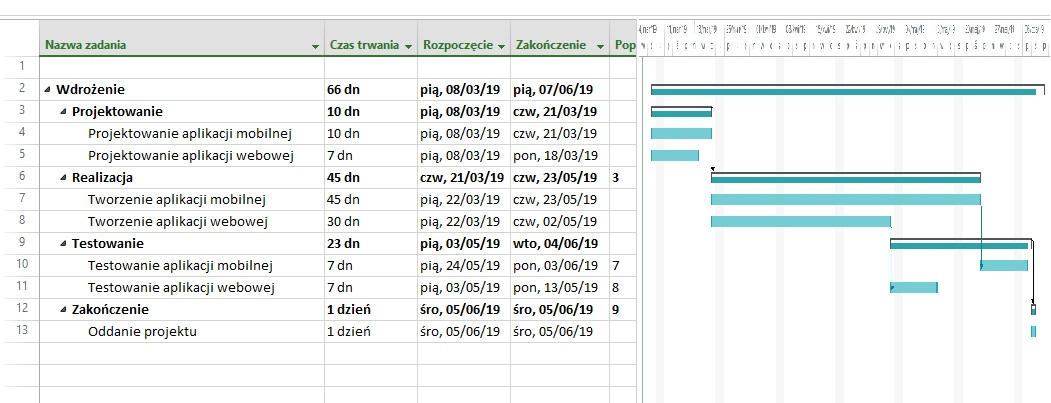
\includegraphics[scale=0.75, angle=270]{wykres_ganttaV3.png}
		\caption{Wykres Gantta}
	\end{figure}
	

Kalkulacja kosztów oraz nakładów pracy potrzebnej do realizacji projektu została przedstawiona w tabeli \ref{kosztorys}.

\begin{table}[H]
\begin{center}
\captionof{table}{Kosztorys}
\label{kosztorys}
	\begin{tabular}{|p{0.55\linewidth}|p{0.15\linewidth}|}%{|l|l|}
	\hline
	Liczba osób 	& 5 				\\ \hline
	Średni czas pracy jednej osoby w godzinach		& 60\\ \hline
	Ilość roboczogodzin & 300	\\ \hline
	Koszt pracy (300h*80zł) & 24000	\\ \hline
	Koszt ubezpieczenia (19.64\%) & 4714	\\ \hline
	Całkowity koszt bezpośredni & \textbf{28714}	\\ \hline
	Koszt pośredni (20\%) & 5743\\ \hline
	Całkowity koszt & 34456\\ \hline
	Zysk & 0\\ \hline
	Podatek VAT (23\%) & 7925\\ \hline
	Koszt produktu & \textbf{42381}\\ \hline
	\end{tabular}
\end{center}
\end{table}


%---------------------------------------------------------
%					Część szósta
%---------------------------------------------------------
\newpage
\section{Opis implementacji i wdrożenia projektu}
(kroki potrzebne by uruchomić / zainstalować projekt + wymagania sprzętowe i programowe)


%---------------------------------------------------------
%					Część siódma
%---------------------------------------------------------
\newpage
\section{Wnioski}

Celem pracy było stworzenie systemu, który będzie umożliwiał w łatwy i wygodny sposób dokumentować historię pojazdów. Wszystkie założenia projektowe zostały spełnione. Podczas realizacji projektu pojawiały się różne trudności, które były na bieżąco rozwiązywane. Jedną z przeszkód było brak darmowego dostępu do API portalu \textit{historiapojazdu.gov.pl}. Ten problem został rozwiązany poprzez stworzenie własnej testowej bazy pojazdów, w której zostały wpisane ręcznie informacje kilku samochodów. Dzięki temu można było przetestować działanie aplikacji.

W przyszłości projekt może zostać w łatwy sposób przerobiony tak, aby odczytywał informacje z portalu \textit{historiapojazdu.gov.pl}, dzięki czemu stanie się w pełni funkcjonalny. Projekt przy odpowiedniej promocji mógłby zostać wdrożony w życie i skomercjalizowany tak, aby przynosił korzyści jego twórcom. Dotychczasowe aplikacje, które są dostępne na rynku nie oferują funkcji potwierdzania autentyczności przebiegu pojazdu. System \textit{Cyfrowej historii pojazdu} oferuje podobne funkcjonalności co rozwiązania konkurencji, jednakże jest rozszerzony o możliwość weryfikacji przebiegu pojazdu. Dzięki temu właściciel pojazdu może poświadczyć autentyczność przebiegu swojego pojazdu, a co za tym idzie zwiększyć jego wartość.


\end{document}


